\documentclass[border=10pt]{standalone}

\usepackage{tikz}
\usetikzlibrary{decorations.markings,calc,arrows}

% Load style for signal-flow graphs
%%%
%%% For the SFGs
%%%
\tikzset{%
	% Style of the node
	Node/.style={circle,thick,draw=black,inner sep=0, minimum size=0.15cm},
	% Style of the node label
	NodeName/.style={font=\footnotesize,black,outer sep=1},
	% Style of the branche label
	ArrowName/.style={font=\footnotesize,auto,outer sep=1},
	% Style of the branch
	Connection/.style={thick},
	->-/.style={decoration={
			markings,
			mark=at position #1 with {\draw[->,>=latex',line width=2pt](0pt,0)--(4pt,0);}},
		postaction={decorate}},
	->-/.default=0.50,
	MarkMiddle/.style={decoration={
			markings,
			mark=at position 0.5 with {\node[NodeName](middle_#1){};}},
		postaction={decorate}},
}

\begin{document}
	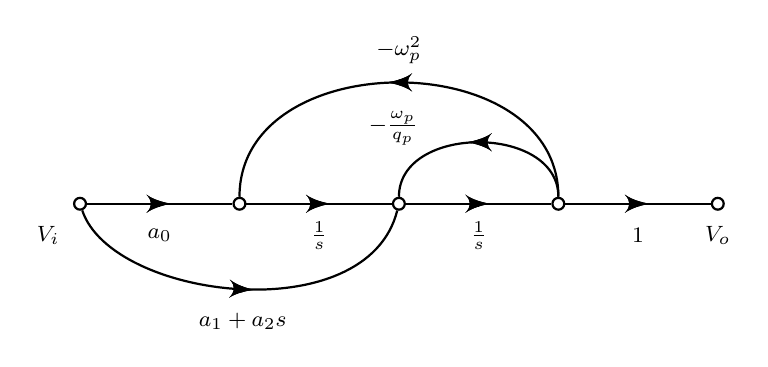
\begin{tikzpicture}[scale = 0.3,x=0.045cm,y=-0.045cm] % STYLES


%~~~~~~~~~~~~~~~~~~~~~~~~~~~~~~~~~~~~~~~~~~~~~~~~~~
% Set Nodes
%~~~~~~~~~~~~~~~~~~~~~~~~~~~~~~~~~~~~~~~~~~~~~~~~~~
\node[Node] (N1) at (630, 270) {};
\node[NodeName] at ($ (N1) + (0, 30) $) {};

\node[Node] (N2) at (480, 270) {};
\node[NodeName] at ($ (N2) + (0, 30) $) {};

\node[Node] (N3) at (180, 270) {};
\node[NodeName] at ($ (N3) + (-30, 30) $) {$V_{i}$};

\node[Node] (N4) at (330, 270) {};
\node[NodeName] at ($ (N4) + (0, 30) $) {};

\node[Node] (N5) at (780, 270) {};
\node[NodeName] at ($ (N5) + (0, 30) $) {$V_{o}$};



%~~~~~~~~~~~~~~~~~~~~~~~~~~~~~~~~~~~~~~~~~~~~~~~~~~
% Set Branches
%~~~~~~~~~~~~~~~~~~~~~~~~~~~~~~~~~~~~~~~~~~~~~~~~~~
%Branch from Node N3 to Node N2
\draw [->-, Connection, MarkMiddle=1] (N3) ..controls(210.0, 360.0) and (450.0, 390.0) .. (N2);
\node[ArrowName] at($ (middle_1) + (0.0, 30.0) $) {$a_{1} + a_{2} s$};

%Branch from Node N1 to Node N2
\draw [->-, Connection, MarkMiddle=2] (N1) ..controls(630.0, 195.0) and (480.0, 195.0) .. (N2);
\node[ArrowName] at($ (middle_2) + (-80.0, -13.0) $) {$- \frac{\omega_{p}}{q_{p}}$};

%Branch from Node N1 to Node N4
\draw [->-, Connection, MarkMiddle=3] (N1) ..controls(630.0, 120.0) and (330.0, 120.0) .. (N4);
\node[ArrowName] at($ (middle_3) + (0.0, -30.0) $) {$- \omega_{p}^{2}$};

%Branch from Node N2 to Node N1
\draw [->-, Connection, MarkMiddle=4] (N2) ..controls(555.0, 270.0) and (555.0, 270.0) .. (N1);
\node[ArrowName] at($ (middle_4) + (0.0, 30.0) $) {$\frac{1}{s}$};

%Branch from Node N4 to Node N2
\draw [->-, Connection, MarkMiddle=5] (N4) ..controls(405.0, 270.0) and (405.0, 270.0) .. (N2);
\node[ArrowName] at($ (middle_5) + (0.0, 30.0) $) {$\frac{1}{s}$};

%Branch from Node N3 to Node N4
\draw [->-, Connection, MarkMiddle=6] (N3) ..controls(255.0, 270.0) and (255.0, 270.0) .. (N4);
\node[ArrowName] at($ (middle_6) + (0.0, 30.0) $) {$a_{0}$};

%Branch from Node N1 to Node N5
\draw [->-, Connection, MarkMiddle=7] (N1) ..controls(705.0, 270.0) and (705.0, 270.0) .. (N5);
\node[ArrowName] at($ (middle_7) + (0.0, 30.0) $) {$1$};



	\end{tikzpicture}
\end{document}